% % ----------------------------------------------------------------------- %
% % Arquivo: 4-proposta-sistema-arquivos.tex
% % ----------------------------------------------------------------------- %

% \chapter{Proposta de Sistema de Armazenamento Distribuído}
% \label{c_proposta}

% A utilização de \textit{data centers} de topologia horizontal e que concentram sua confiabilidade em \textit{software} é vasta. Os \textit{data centers} da Google, por exemplo, possuem topologia horizontal. De acordo com \citeonline{googledatacenter}, isto ocorre por dois motivos, sendo o primeiro a melhor relação entre custo e desempenho oferecida pela topologia horizontal, tendo uma infraestrutura de computação suportada em \textit{hardware} de baixa confiabilidade e custo (como computadores pessoais), e a segunda a otimização dos serviços ofertados, alcançada através da paralelização de processamento de requisições ao invés de tempo de resposta e performance individual de servidores. Na prática, isto significa que a Google confia que o \textit{software} utilizado em seu \textit{data center} provê tanto o grau de confiabilidade necessário para ofertar seus serviços quanto o melhor cenário de otimização para os serviços implantados. O Facebook, por sua vez, também possui uma topologia de rede horizontal, similar a topologia \ac{ToR} \cite{facebookdatacenter}.

% As topologias horizontais utilizadas em ambas, Google e Facebook, permitem que contêineres sejam utilizados em suas infraestruturas para implantar serviços. No Facebook é utilizado o Tupperware, um orquestrador de contêineres proprietário desenvolvido pela própria empresa \cite{facebookcontaineres}. Já na Google a orquestração de contêineres é realizada através do gerenciador de \textit{cluster} Borg \cite{googleborg}, sendo que desde 2014 a Google já executava todos os seus serviços em formato de contêineres \cite{googleslides}. Em 2014, por exemplo, 2 bilhões de contêineres eram criados semanalmente nos \textit{data centers} da Google \cite{googleslides}.

% Nuvens de computação de menor escala também podem usufruir das vantagens de contêineres, principalmente ao utilizar um orquestrador como o Kubernetes, por exemplo. A eficiência do Kubernetes é reconhecida pela sua implementação em nuvens públicas, como na \ac{AWS} e \ac{GCP}. Um exemplo de empresa que utiliza o Kubernetes através da \ac{Amazon EKS} para implantação de serviços é a GoDaddy \cite{godaddyeks}. Já um exemplo de organização que utiliza o Kubernetes em sua nuvem privada e local é a \ac{CERN} \cite{cernk8s}. Outro exemplo de organização que está utilizando o Kubernetes é o \ac{Serpro}, que está trabalhando no projeto Estaleiro desde o fim de 2016 para oferecer um ambiente ideal para o desenvolvimento e operação dos produtos e serviços da empresa \cite{serproestaleiro}.

% Considerando a infraestrutura ideal descrita no capítulo anterior, a atual infraestrutura de serviços presente no \ac{IFSC} e as tecnologias atualmente utilizadas por empresas de destaque como a Google e o Facebook, propõe-se a criação de uma nuvem de contêineres distribuída nos câmpus do \ac{IFSC} para fornecimento de serviços e armazenamento de dados da instituição. A escolha de múltiplos câmpus para composição da nuvem dá-se pelos seguintes motivos: georreplicação e alta disponibilidade de dados e serviços devido à descentralização da infraestrutura, adoção de topologia horizontal, a qual facilita a expansão do sistema e heterogeneidade dos componentes nele utilizados, e descentralização da gestão de serviços, a qual permite que mais funcionários da instituição estejam envolvidos na expansão e manutenção do sistema. Também considerando a capacidade computacional de cada câmpus do \ac{IFSC} e as taxas de transmissão disponível, propõe-se que a infraestrutura de serviços seja distribuída nos câmpus do \ac{IFSC} de São José, Florianópolis (Mauro Ramos) e na Reitoria. Estes três câmpus formariam um anel, provendo serviços e armazenamento de dados de forma conjunta, como mostrado na \autoref{ifsc_cloud}.

% % Como resultado da descentralização da infraestrutura propõe-se a implantação de uma infraestrutura de serviços de topologia horizontal, a qual resultará na heterogeneidade dos componentes utilizados nos \textit{data centers}. Isto significa que caso seja necessário expandir ou reparar o sistema a especificação dos componentes necessários para ampliação poderá ser muito mais genérica, não sendo necessário realizar a aquisição de \textit{hardware} proprietário, específico e de alto custo. Será possível, portanto, utilizar \textit{hardware} de menor custo e de diferentes fabricantes nos \textit{data centers}. Isto é realizável pela utilização de protocolos comuns entre os \textit{softwares} utilizados, abandonando assim a necessidade de utilização de \textit{hardware} comum no \textit{data center}.

% \begin{figure}[!htpb]
% 	\centering
% 	\caption{Infraestrutura de serviços proposta}
%     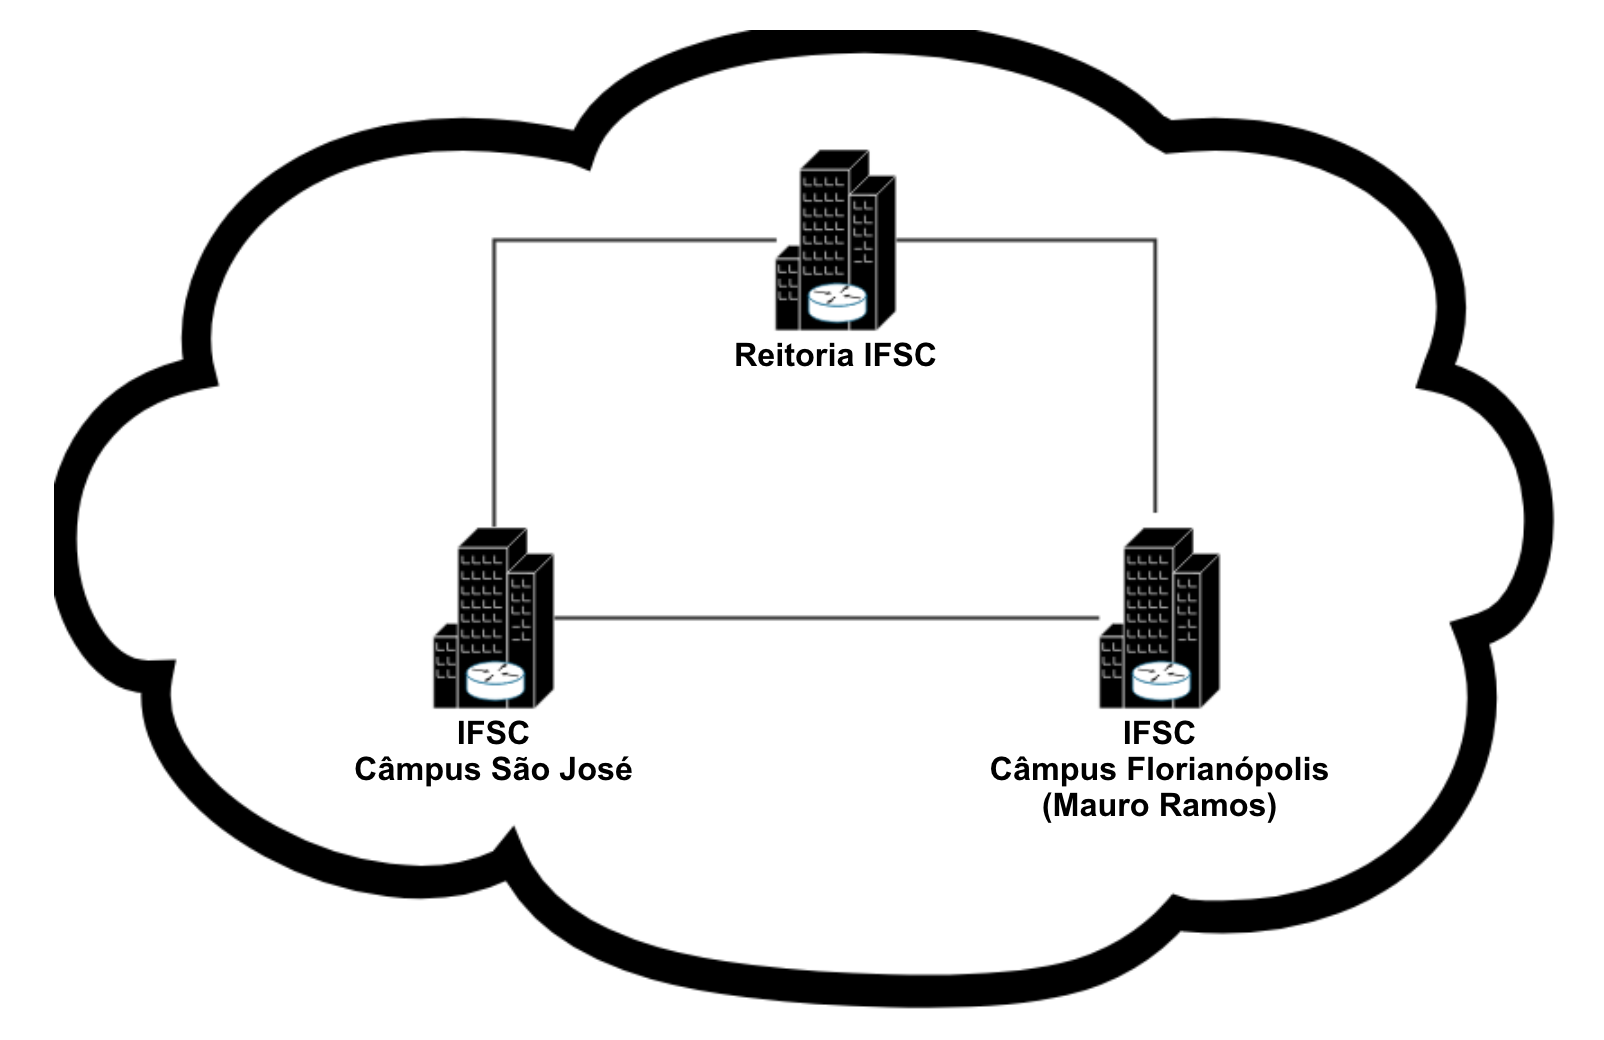
\includegraphics[width=14cm]{TCC/figuras/4-proposta/IFSC-Cloud}
    
% 	Fonte: Elaborado pelo autor.
%  	\label{ifsc_cloud}
% \end{figure}

% Do ponto de vista de armazenamento de dados, os dados da instituição estarão armazenados em múltiplas regiões (isto é, em câmpus distintos), aumentando a replicação destas informações e diminuindo assim o risco de perda de informações devido a pontos únicos de falha no sistema. Isto pode ser exemplificado, por exemplo, por um desastre de interrupção \textbf{local} do serviço em um dos câmpus da instituição. Mesmo que os dados armazenados no câmpus sejam perdidos os mesmos estarão disponíveis em outros câmpus. O sistema de armazenamento sugerido neste trabalho, Ceph, permite que \textit{backups} de dados sejam realizados de diversas formas. Dentre estas formas destacam-se a replicação de dados para outro \textit{cluster} Ceph (\textit{Ceph-on-Ceph}) e \textit{snapshots} geradas pelo sistema de armazenamento \cite{cephbackup}. Além disso, o Rook, plataforma de armazenamento que automatiza a utilização do Ceph em \textit{clusters} Kubernetes, também possibilita outras alternativas de \textit{backup}, como cópia dos dados armazenados nos volumes utilizados por contêineres, por exemplo.

% A descentralização da infraestrutura aumenta também a tolerância a falha dos serviços, pois, como explicado, os serviços fornecidos pela instituição também estarão disponíveis em múltiplas regiões, diminuindo assim a probabilidade destes ficarem indisponíveis devido a incidentes regionais em cada câmpus, como panes elétricas ou instabilidade nos enlaces de conexão da instituição, por exemplo.

% A expansão da infraestrutura de serviços para outros câmpus facilitará também a transição do modelo de gestão de serviços e \ac{TI} no \ac{IFSC} para um modelo mais descentralizado e colaborativo. Isto significa que funcionários de outros câmpus também poderão participar da manutenção e gestão efetiva dos serviços e infraestrutura da instituição. Este modelo de gestão descentralizada permitirá que não apenas mais pessoas participem na manutenção do sistema, mas também que funcionários que possuam interesse em trabalhar com a gestão deste sistema tenham esta oportunidade. Esta é, portanto, uma proposta que envolve não apenas a reestruturação da infraestrutura de serviços da instituição, mas também uma proposta de remodelagem de gestão de \ac{TI} no \ac{IFSC}.

% A implantação desta infraestrutura descentralizada poderá ocasionar a necessidade de adoção de outras tecnologias que garantam o funcionamento do sistema de forma eficiente. A utilização de \ac{QoS} na rede federada ou estabelecimento de \textit{caches} para armazenamento de dados frequentemente acessados em outros câmpus são exemplos de tecnologias que devem ser levadas em consideração. Entretanto, tais necessidades poderão ser apenas confirmadas e/ou efetivamente consideradas na implantação do sistema e em testes para verificação de seu desempenho.

% % Considerando a capacidade de processamento atual da instituição, tendências tecnológicas e \textit{hardware} legado e atual, propõe-se que a infraestrutura de serviços da instituição consista em uma nuvem de contêineres. Contêineres podem ser gerenciados através de um orquestrador de contêineres, como o Kubernetes, por exemplo. Um orquestrador de contêineres permite a rápida implantação e gestão de serviços. A implantação de novos serviços através de contêineres é facilitada pois os próprios contêineres já possuem grande parte dos conteúdos (bibliotecas e códigos) necessários para sua execução, sem precisar que todo o ambiente seja configurado especificamente para sua execução. O orquestrador também facilita a manutenção dos serviços, haja vista que regras de reinicialização de contêineres, escalabilidade e tratamento de erros podem ser facilmente configurados. Contêineres são amplamente utilizados por empresas para prover serviços internos ou externos.   

% Contêineres são uma ótima alternativa para prover serviços. Entretanto, antes de discutir a implementação de serviços em uma nuvem, é necessário que se defina como os dados e informações desta nuvem serão armazenados. Isto ocorre pois estes serviços estarão armazenando dados, e esta camada inferior deve ser primeiro definida e estudada para que seja então possível a implantação dos serviços. No contexto do \ac{IFSC} propõe-se a hiperconvergência de infraestrutura, ou seja, propõe-se que tanto que processamento e armazenamento sejam realizados na mesma infraestrutura de contêineres. Mais detalhes sobre esta proposta estão descritas a seguir.


% % ----------------------------------------------------------------------- %
% \section{Sistema de armazenamento distribuído}

% Sistemas de armazenamento são utilizados para armazenar desde arquivos pessoais até bases de dados, páginas \textit{Web} e credenciais de acesso. O sistema de armazenamento utilizado determina como será o acesso aos dados armazenados em disco, possibilitando assim que a aplicação em execução não seja responsável por armazenar diretamente o arquivo em disco, os quais são gerenciados pelo sistema de arquivos.

% No contexto da infraestrutura de serviços proposta para o \ac{IFSC}, sistemas de armazenamento distribuídos também possuem um papel central na concepção do sistema. Isto ocorre por dois motivos principais, sendo o primeiro a limitação de recursos computacionais disponíveis e o segundo a utilização de uma nuvem de contêineres. O primeiro motivo é simples: diferentemente de grandes \textit{data centers}, o \ac{IFSC} possui uma baixa capacidade de escalabilidade a curto prazo devido a pequena margem de folga dos recursos computacionais disponíveis, tornando difícil a utilização de parte destes recursos exclusivamente para armazenamento. Isto significa que, caso o armazenamento e processamento fossem realizados separadamente, seria necessário realizar a divisão de \textit{hardware} entre armazenamento e processamento, o que poderia deixar uma destas áreas deficitária. Já o segundo motivo, que é a utilização de contêineres, destaca-se como uma alternativa que permite que ambos, armazenamento e processamento, sejam realizados no mesmo \textit{hardware}, mas logicamente separados. Esta abordagem é emergente e estudos e projetos têm sido desenvolvidos para tornar a implementação de sistemas de armazenamento distribuídos viável neste contexto, sendo o termo hiperconvergência utilizado para caracterizar a oferta de armazenamento e processamento em \textit{hardware} comum e logicamente separado por \textit{software} \cite{vmwarehyperconvergence}.

% Um sistema de armazenamento distribuído amplamente utilizado é o Ceph. Exemplos de organizações que utilizam o Ceph são: \textit{Western Digital}, \ac{CERN}, Cisco e \textit{Digital Ocean} \cite{cephusers}. Este sistema de armazenamento permite o armazenamento de dados através de objetos, arquivos e blocos. O Ceph é um sistema de armazenamento distribuído altamente flexível, redundante, eficiente e configurável. Ele é, entretanto, complexo tanto em sua implantação quanto manutenção. Há ferramentas que automatizam a utilização do Ceph. Entre estas ferramentas, destaca-se o Rook, uma plataforma de armazenamento para Kubernetes, ou seja, uma plataforma que pode ser utilizada na nuvem de contêineres proposta para o \ac{IFSC}. O Rook é um projeto de código livre iniciado em 2016 e que está atualmente na incubadora da \ac{CNCF} \cite{rookhistory}.

% Apesar de ainda estar em desenvolvimento durante o decorrer deste trabalho, o Rook provou ser uma solução de armazenamento que pode ser utilizada no \ac{IFSC}. Ao automatizar a implementação do Ceph esta plataforma de armazenamento permite tanto o armazenamento de dados persistentes (como bancos de dados) e de arquivos com baixa taxa de atualização (como páginas \textit{Web} e imagens, por exemplo). Esta automatização possibilita a implantação do Ceph em \textit{clusters} de contêineres e permite que a replicação, redundância e outras funcionalidades do Ceph sejam todas configuradas e aplicadas de maneira fácil e transparente no \textit{cluster}.

% O próximo capítulo mostrará a implementação do Rook em um \textit{cluster} Kubernetes para provisionamento de arquivos através de blocos de armazenamento e objetos. Os blocos de armazenamento são utilizados para armazenamento de dados persistentes dos contêineres, enquanto o armazenamento de objetos é utilizado para prover arquivos estáticos (neste caso, imagens). Esta implementação foi realizada na \ac{GCP} devido à falta de \textit{hardware} disponível no câmpus para utilização no trabalho. Para manter a implementação o mais fiel possível a um cenário real foram utilizadas máquinas virtuais ao invés da \ac{API} de gerenciamento de \textit{clusters} Kubernetes disponível na plataforma da Google. Foram utilizadas apenas três máquinas virtuais para validação do modelo, que também pode ser reproduzido em um cenário de maior escala. Detalhes da criação da infraestrutura remota, implementação do \textit{cluster} Kubernetes e provisionamento de arquivos estão detalhados no capítulo a seguir.